% Chapter Template

\chapter{Ensayos y resultados} % Main chapter title

\label{Chapter4} % Change X to a consecutive number; for referencing this chapter elsewhere, use \ref{ChapterX}

%----------------------------------------------------------------------------------------
%	SECTION 1
%----------------------------------------------------------------------------------------
En este capítulo se explica la metodología de pruebas aplicada tanto a los componentes individuales como al sistema implementado para finalizar con una comparación con el estado del arte.


\section{Banco de pruebas}
\label{sec:Banco de pruebas}
%
La verificación del correcto funcionamiento de los módulos que componen el sistema se realizó mediante una maqueta que se muestra en la figura \ref{fig:maqueta} y representa en escala reducida al invernadero del cliente.

El modelo cuenta con una bomba de agua conectada a tres válvulas para alimentar a los circuitos de riego. 
Se utilizaron mangueras y conexiones neumáticas de aluminio de acople rápido y el conjunto armado puede verse en la figura \ref{fig:pump}. 
  
El ensamblado se muestra en las figuras \ref{fig:gh1}, \ref{fig:gh2} y \ref{fig:gh3} donde se observa la implementación de dos circuitos de riego independientes. También se configuró un tercer circuito cerrado para pruebas de accionamiento de bomba y válvula a fin de evitar desperdicios durante las fases de calibración.


\begin{figure}[h]
	\centering
	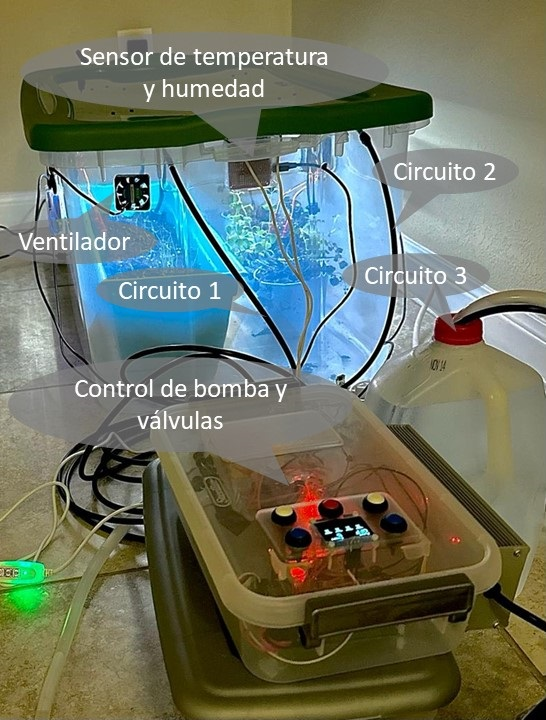
\includegraphics[width=0.50\textwidth]{./Figures/chapter4/maqueta.jpg}
	\caption[Modelo completo del invernadero]{Modelo completo del invernadero.}
	\label{fig:maqueta}
\end{figure}

Además se incorporaron a la maqueta dos módulos sensores de humedad del suelo, uno de temperatura y humedad y un actuador para el encendido de los ventiladores.

Para las pruebas manuales de accionamiento de los diferentes sistemas se empleó una computadora portátil y un celular para las pruebas de acceso concurrente a la aplicación central.

\begin{figure}[htpb]
     \centering
       \begin{subfigure}[b]{0.45\textwidth}
	    \centering
		 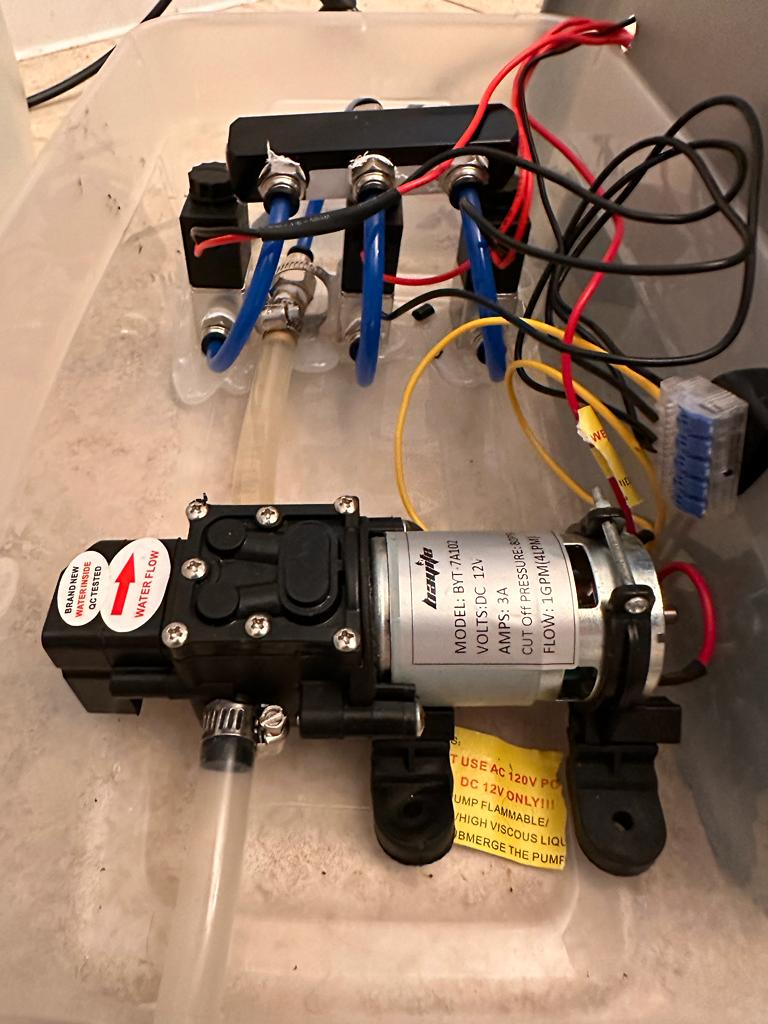
\includegraphics[width=0.75\textwidth]{./Figures/chapter4/pump_2.jpg}
		\caption{Conjunto bomba y válvulas.}
		\label{fig:pump}
     \end{subfigure}
          \hfill
     \begin{subfigure}[b]{0.45\textwidth}
		\centering
		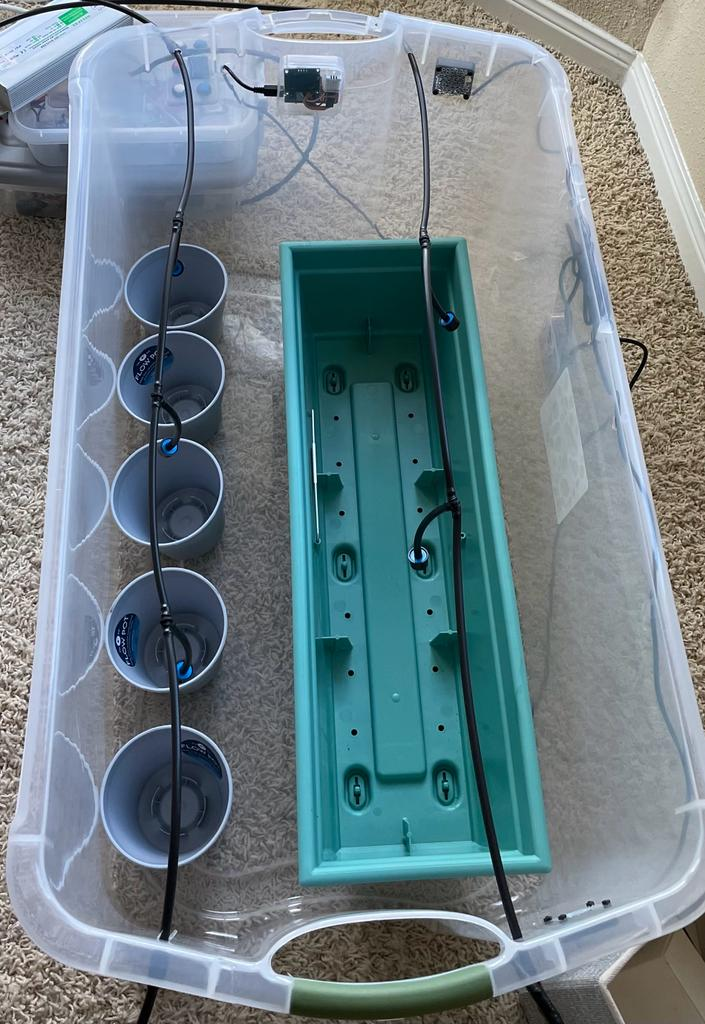
\includegraphics[width=0.70\textwidth]{./Figures/chapter4/Invernadero1.jpg}
		\caption{Armado de mangueras de riego.}
		\label{fig:gh1}
     \end{subfigure}
     \hfill
     \begin{subfigure}[b]{0.45\textwidth}
	    \centering
		 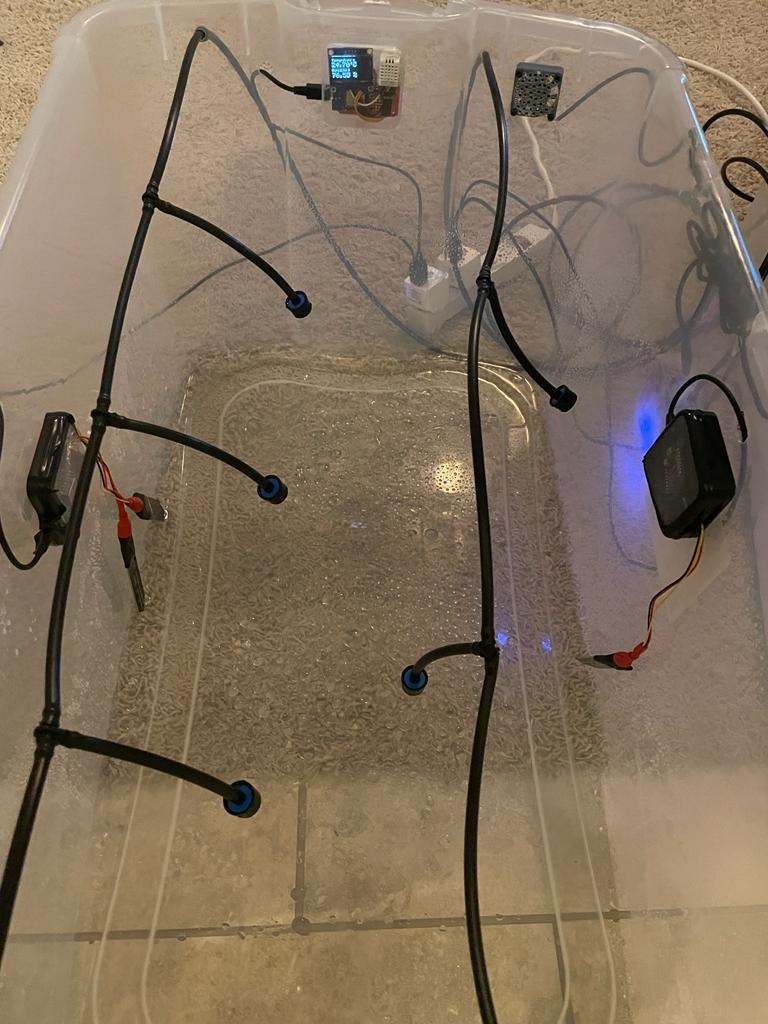
\includegraphics[width=0.75\textwidth]{./Figures/chapter4/Invernadero2.jpg}
		\caption{Pruebas de riego.}
		\label{fig:gh2}
     \end{subfigure}
     \hfill	
	 \begin{subfigure}[b]{0.45\textwidth}
		\centering
		\includegraphics[width=0.65\textwidth]{./Figures/chapter4/Invernadero3.jpg}
		\caption{Ensamble general.}
		\label{fig:gh3}
     \end{subfigure}
     \hfill

        \caption[Modelo de pruebas del invernadero]{Modelo de pruebas del invernadero.}
        \label{fig:invernadero}
\end{figure}



\pagebreak
\section{Pruebas individuales}
\label{sec:Pruebas individuales}

Se detallan las principales pruebas realizadas a los módulos a fin de garantizar su correcto funcionamiento y/o el cumplimiento de requerimientos.


\subsection{Pruebas a módulos sensores}
\label{sec:Pruebas a módulos sensores}

\begin{itemize}
\item Conexión a los sensores y valores obtenidos: Se conectaron individualmente los módulos a la computadora mediante la consola serial de Arduino IDE y se constataron los valores obtenidos frente a cambios inducidos sobre la magnitud a medir.

\item Resistencia al agua y a salpicaduras: Requerimiento no funcional explícito para los sensores de humedad del suelo. Consistió en comprobar la integridad y el funcionamiento del módulo al tiempo que se sumergía el sensor en un recipiente con agua o se lo sometía a aspersiones continuas por alrededor de 30 segundos con atomizadores desde diferentes ángulos.
La figura \ref{fig:soil_test} esquematiza parcialmente el proceso de prueba mencionado.

  
\end{itemize}


\begin{figure}[h]
	\centering
	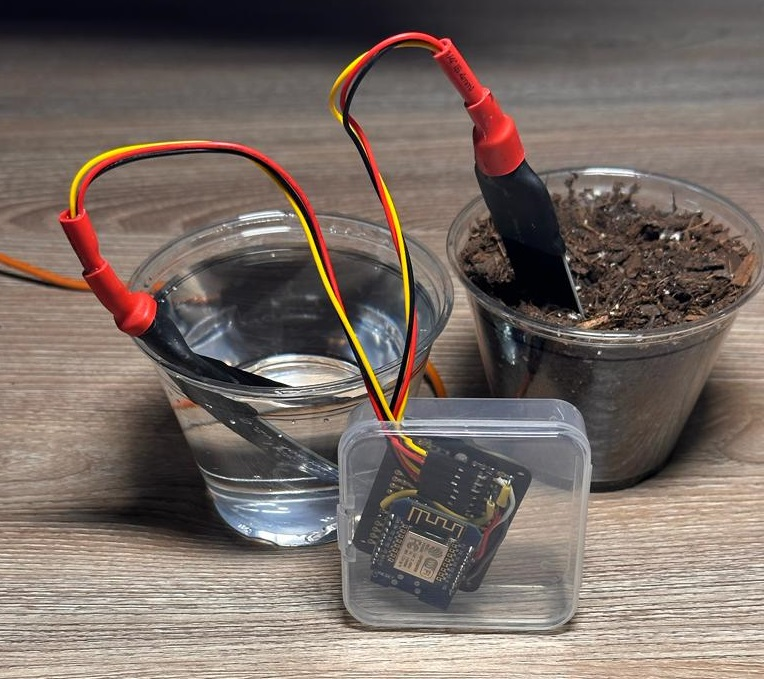
\includegraphics[width=0.50\textwidth]{./Figures/chapter4/soil_testing3.jpg}
	\caption[Prueba de resistencia al agua]{Prueba de resistencia al agua.}
	\label{fig:soil_test}
\end{figure}

\subsection{Pruebas a módulos actuadores}
\label{sec:Pruebas a módulos actuadores}

Se conectaron las salidas de los pines de GPIO a leds para visualizar el encendido y apagado del actuador. 

Se desarrolló una interfaz simple en ThingsBoard a fin de enviar las señales de comando al módulo La aplicación por medio de mensajes RPC sobre MQTT. El microcontrolador recibe la orden y ejecuta la acción, reflejada en el estado de los leds correspondientes.



\begin{figure}[htpb]
     \centering
       \begin{subfigure}[b]{0.50\textwidth}
	    \centering
		 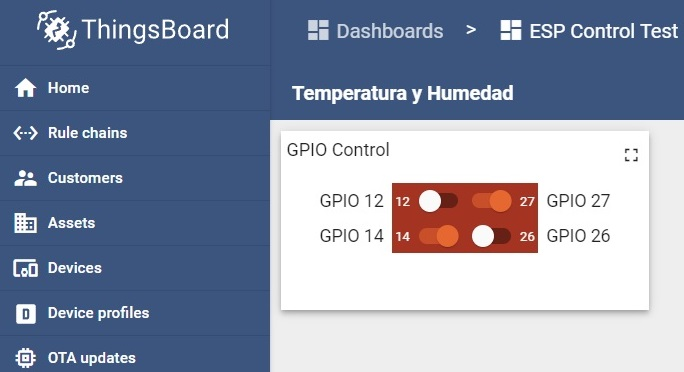
\includegraphics[width=0.9\textwidth]{./Figures/chapter4/control_unit_test_1.jpg}
		\caption{Ventana de control.}
		\label{fig:control_test1}
     \end{subfigure}
          \hfill
     \begin{subfigure}[b]{0.45\textwidth}
		\centering
		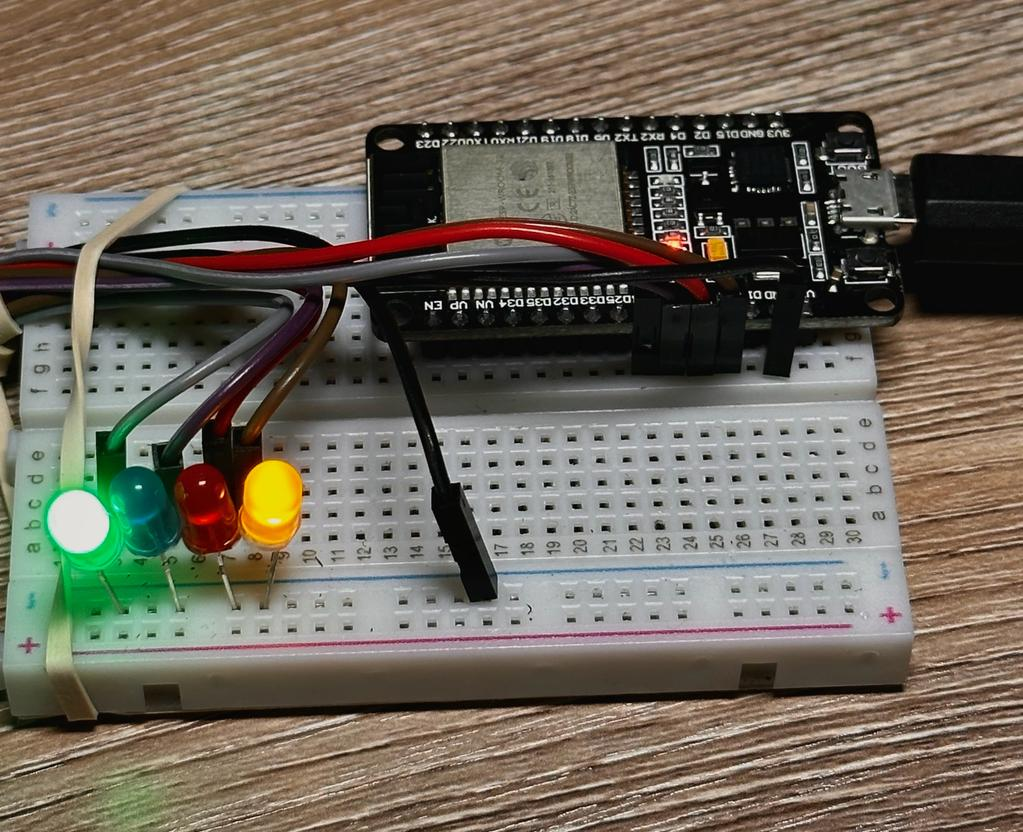
\includegraphics[width=0.70\textwidth]{./Figures/chapter4/control_test2.jpg}
		\caption{Verificación del actuador mediante leds.}
		\label{fig:control_test2}
     \end{subfigure}
     \hfill
        \caption[Pruebas unitarias sobre controladores]{Pruebas unitarias sobre controladores.}
        \label{fig:control_test}
\end{figure}


\subsection{Pruebas de acceso concurrente a la aplicación}
\label{sec:Pruebas de acceso concurrente a la aplicación}



Las pruebas de concurrencia se efectuaron mediante el acceso simultáneo de diferentes usuarios mediante una computadora portátil y un teléfono celular. Los ensayos consistieron en realizar diferentes acciones desde un dispositivo como, por ejemplo, el accionamiento de un circuito de riego por parte de un usuario, y la confirmación del cambio de estado recibida por otro. 
 
La figura \ref{fig:tb_compu} muestra la vista obtenida mediante el uso del ordernador mientras que la figura  \ref{fig:tb_celu} la del celular.

\begin{figure}[htpb]
     \centering
       \begin{subfigure}[b]{0.53\textwidth}
	    \centering
		 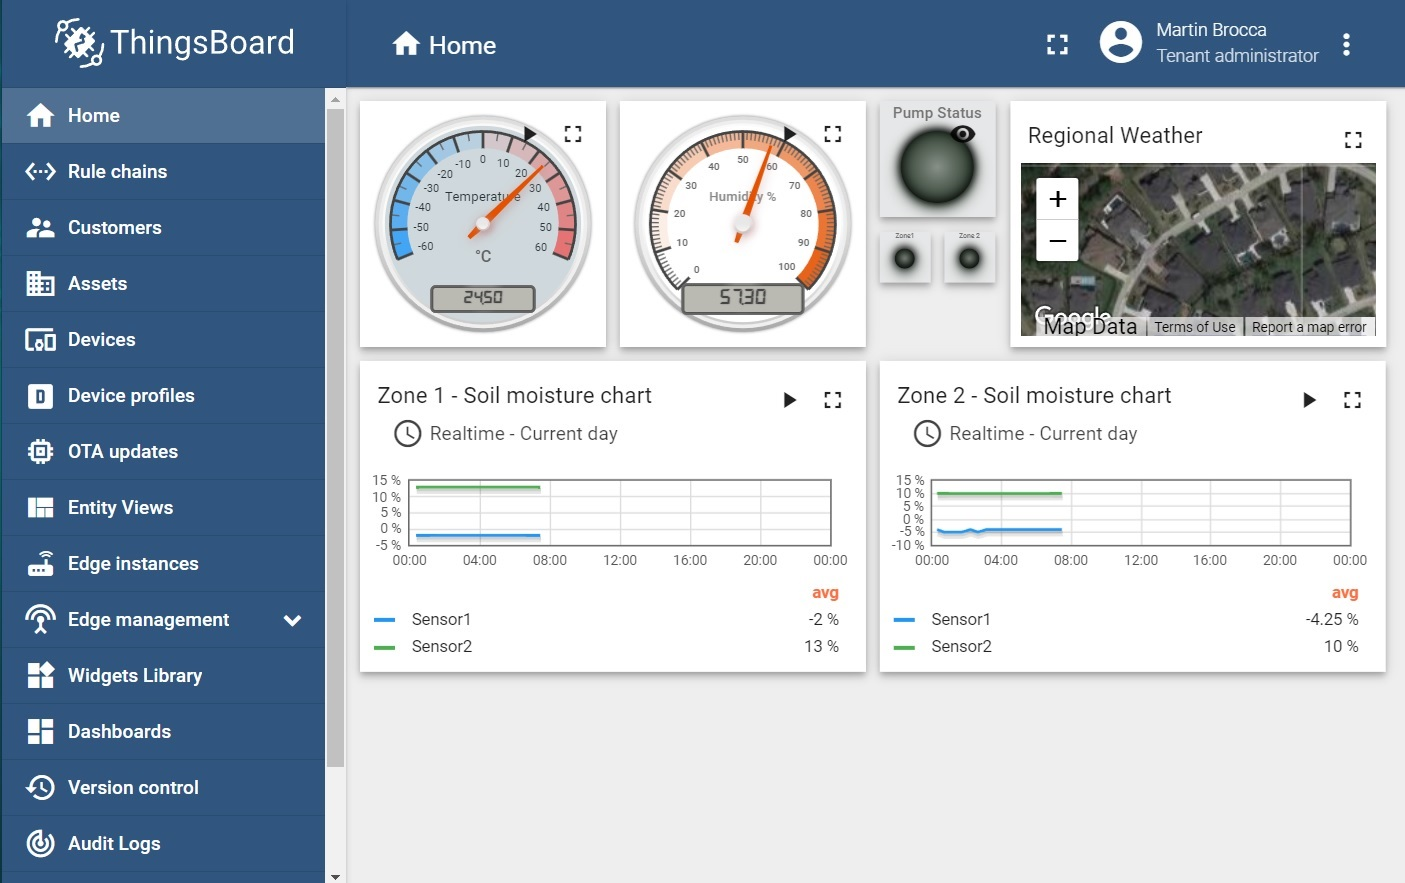
\includegraphics[width=0.9\textwidth]{./Figures/chapter4/tb_compu.jpg}
		\caption{Vista sobre acceso por computadora.}
		\label{fig:tb_compu}
     \end{subfigure}
          \hfill
     \begin{subfigure}[b]{0.45\textwidth}
		\centering
		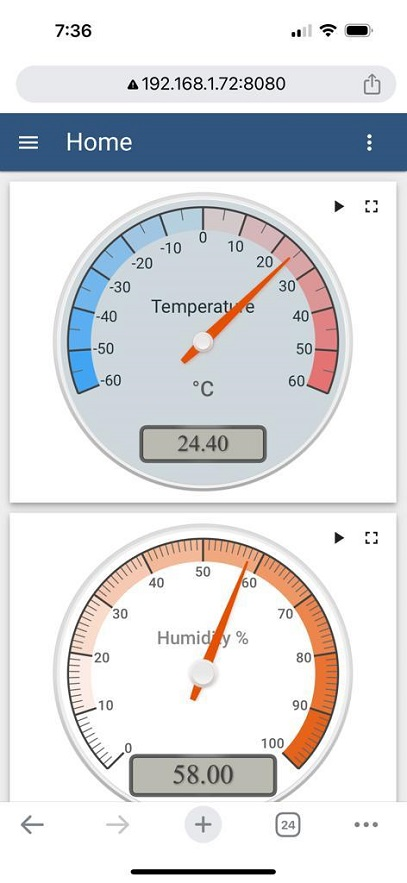
\includegraphics[width=0.40\textwidth]{./Figures/chapter4/tb_celu.jpg}
		\caption{Vista sobre acceso por teléfono celular.}
		\label{fig:tb_celu}
     \end{subfigure}
     \hfill
        \caption[Pruebas unitarias sobre acceso concurrente]{Pruebas unitarias sobre acceso concurrente.}
        \label{fig:tb_concurrencia}
\end{figure}

\section{Pruebas de sistema}
\label{sec:Pruebas de sistema}

El objetivo de las pruebas de integración es verificar el correcto funcionamiento e interacción de los sistemas que conforman el modelo. Para este propósito se desarrollaron reglas de automatización para el control de riego y de temperatura, además de las necesarias para el manejo de alarmas del sistema. 

Las reglas de control son similares en construcción y consisten en un nodo de espera de mensajes, seguido de un filtro de información para capturar la telemetría de los sensores. Esta es comparada con un valor de referencia configurado en la aplicación, y conforme se cumpla la condición se dispara una alerta de notificación al cliente y se informa al actuador que comience una acción. Si la comparación resultase negativa, se limpia cualquier alerta presente, se verifica si hay que frenar al actuador, y se retorna al comienzo.
El esquema de una regla de control genérica puede verse en la fig \ref{fig:basic_rule}.

\begin{figure}[h]
	\centering
	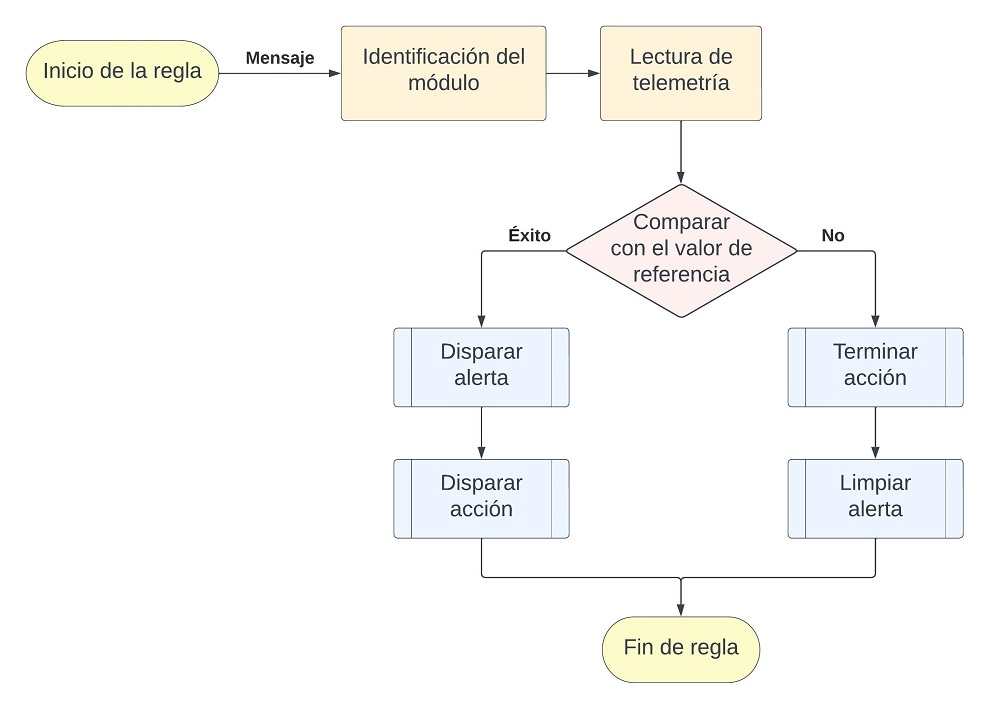
\includegraphics[width=0.6\textwidth]{./Figures/chapter4/ReglaBasica.jpg}
	\caption[Regla de automatización genérica]{Regla de automatización genérica.}
	\label{fig:basic_rule}
\end{figure}

\pagebreak

\subsection{Control de clima}
\label{sec:Control de clima}

Se definió una regla de control con un límite máximo de 28 °C de temperatura que cuando se supera, realiza el envío de un mensaje de encendido de ventiladores y dispara una notificación al usuario. Cuando la temperatura se mantiene por debajo del umbral, se cancelan las alarmas y se retorna al estado de espera de mensajes. La regla implementada puede verse en la figura \ref{fig:temp_rule}.  

\begin{figure}[h]
	\centering
	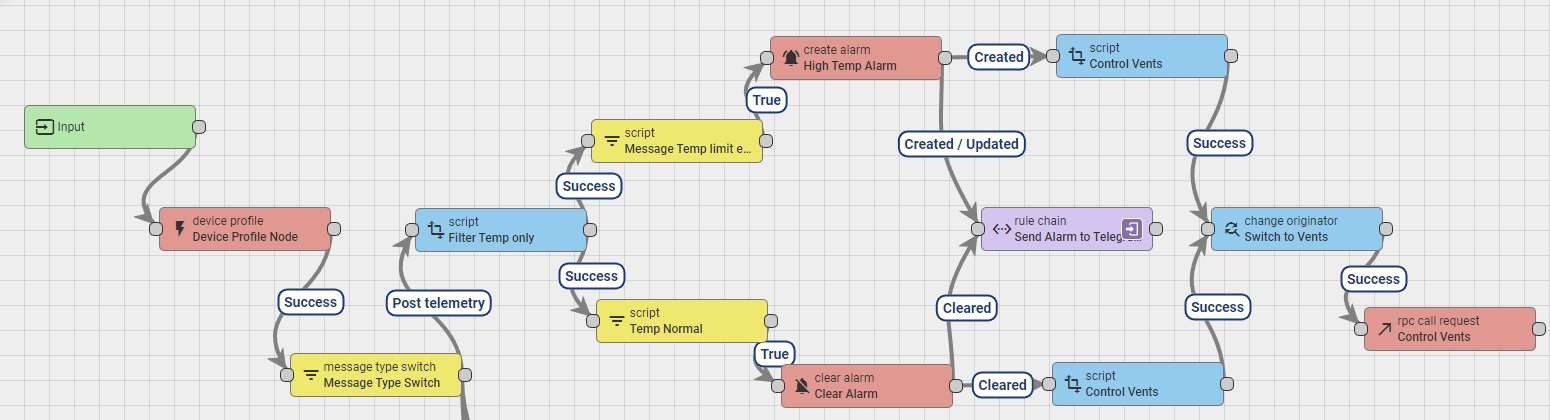
\includegraphics[width=1\textwidth]{./Figures/chapter4/temp_rule.jpg}
	\caption[Regla de control de clima]{Regla de control de clima.}
	\label{fig:temp_rule}
\end{figure}

Para la prueba se procedió a incrementar la temperatura artificialmente por medio de una pistola de calor y observar la reacción del sistema. La figura \ref{fig:temp_graph} indica el punto donde el cambio de temperatura dispara la acción del sistema y se encendieron los ventiladores, mientras que en la figura \ref{fig:temp_alarm} se indica la alarma creada por este evento.  







%\begin{figure}[h]
%	\centering
%	\includegraphics[width=0.7\textwidth]{./Figures/chapter4/ventrule.jpg}
%	\caption[Regla de automatización de ventilador]{Regla de automatización de ventilador.}
%	\label{fig:temp_rule}
%\end{figure}


\begin{figure}[htpb]
     \centering
       \begin{subfigure}[b]{0.8\textwidth}
	    \centering
		 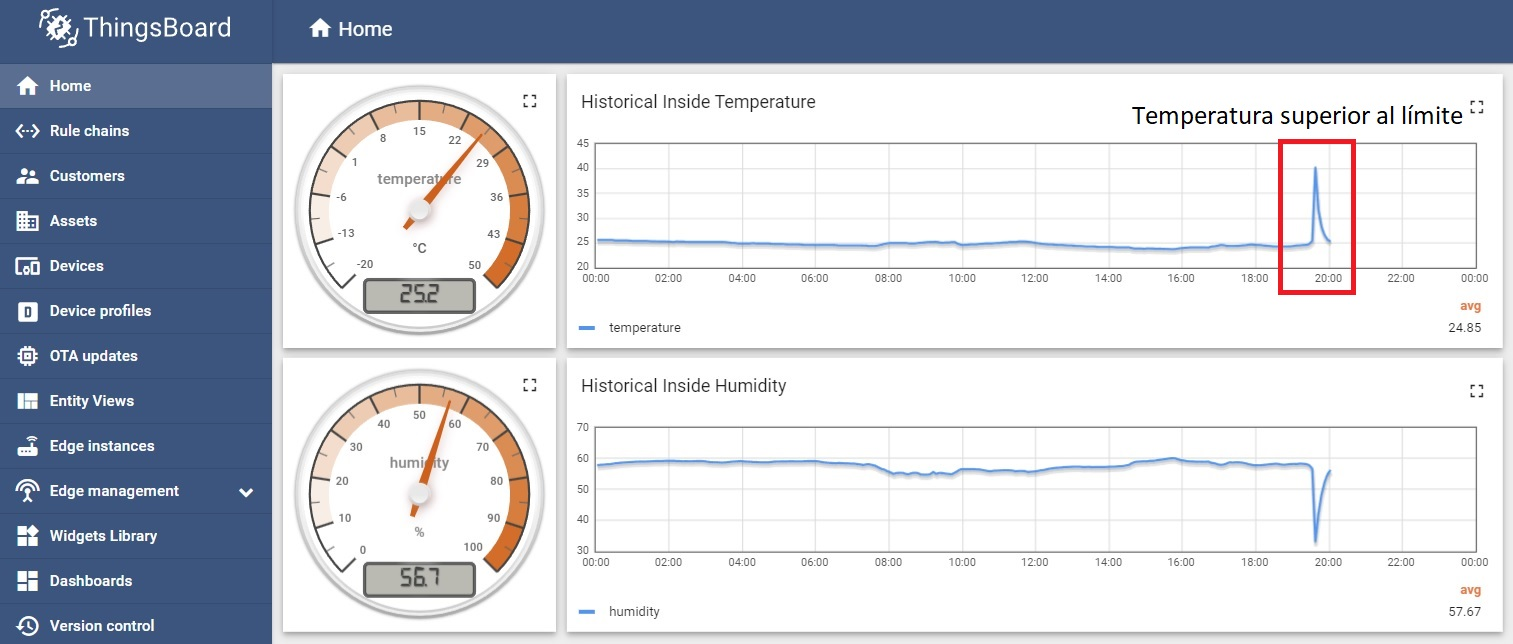
\includegraphics[width=0.9\textwidth]{./Figures/chapter4/temperature.jpg}
		\caption{Vista del historial de temperatura.}
		\label{fig:temp_graph}
     \end{subfigure}
          \hfill
     \begin{subfigure}[b]{0.80\textwidth}
		\centering
		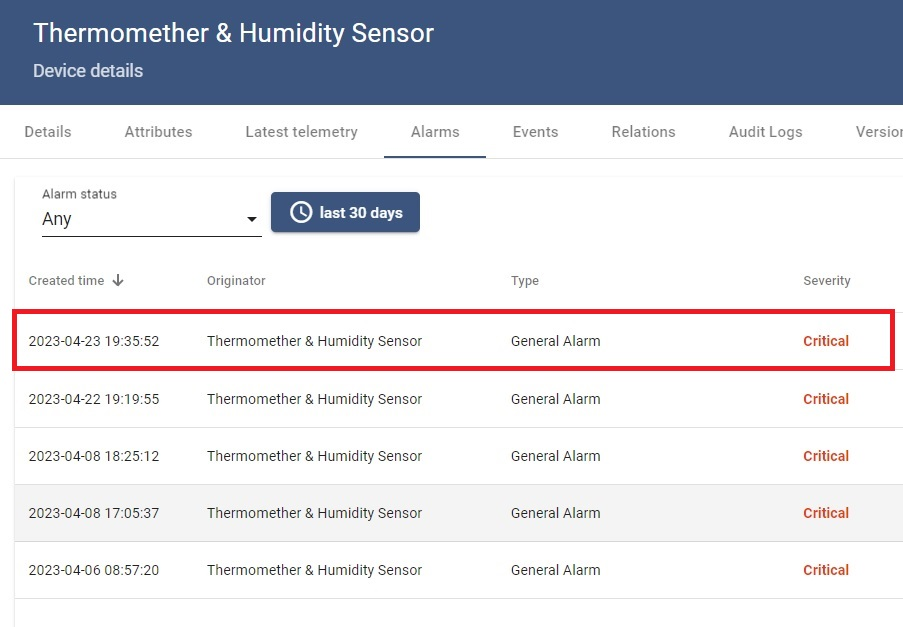
\includegraphics[width=0.80\textwidth]{./Figures/chapter4/temp_alarm.jpg}
		\caption{Alarmas generadas al superar los límites.}
		\label{fig:temp_alarm}
     \end{subfigure}
     \hfill
        \caption[Generación de alarmas por exceso de temperatura]{Generación de alarmas por exceso de temperatura.}
        \label{fig:tb_concurrencia}
\end{figure}


\pagebreak
\subsection{Control de riego}
\label{sec:Control de riego}

La prueba de integración del sistema de riego consistió de una regla de control en la que se reciben mensajes de lectura de valores provenientes de los sensores de humedad del suelo. Como primer paso, se identifica la zona a la que pertenecen las sondas y luego se evalúa la telemetría contra un valor de referencia. Si el valor es inferior al definido, lo que indica un suelo seco, se debe iniciar el sistema de bomba y válvula correspondiente al circuito por el tiempo de riego predefinido. 

Para evaluar la regla se plantearon los siguientes parametros de configuración:
\begin{itemize}
\item Sensor seco: Sonda expuesto al aire, limpio y sin rastros de humedad.
\item Sensor saturado: Sensor introducido un recipiente con agua.
\item Sensor húmedo: Sensor introducido en tierra húmeda con una humedad aproximada del 30%
\end{itemize}

%\begin{tabular}{lllllll}
%\toprule
%\multicolumn{2}{l}\textbf{Zona 1}      & \multicolumn{2}{l}\textbf{Zona 2}        & \textbfRiego 1 & \textbf{Riego} 2 & \textbf{Resultado} \\
%\midrule
%Sensor seco   & Sensor saturado & Sensor saturado & Sensor saturado & No      & No      & OK        \\
%Sensor seco   & Sensor seco     & Sensor saturado & Sensor saturado & Sí      & No      & OK        \\
%Sensor seco   & Sensor saturado & Sensor seco     & Sensor saturado & No      & No      & OK        \\
%Sensor seco   & Sensor saturado & Sensor seco     & Sensor seco     & No      & Si      & OK        \\
%Sensor seco   & Sensor húmedo   & Sensor seco     & Sensor húmedo   & No      & No      & OK        \\
%Sensor húmedo & Sensor húmedo   & Sensor húmedo   & Sensor húmedo   & No      & No      & OK        \\
%Sensor húmedo & Sensor húmedo   & Sensor seco     & Sensor seco     & No      & Si      & OK  
%\bottomrule
%\hline
%\end{tabular}
%\label{tab:riego_test}
%\end{table}

\begin{table}[]
\begin{tabular}{lllllll}
\hline
\multicolumn{2}{l}{\textbf{Zona 1}} & \multicolumn{2}{l}{\textbf{Zona 2}} & \textbf{Riego 1} & \textbf{Riego 2} & \textbf{Resultado} \\ \hline
Sensor seco   & Sensor saturado & Sensor saturado & Sensor saturado & No & No & OK \\
Sensor seco   & Sensor seco     & Sensor saturado & Sensor saturado & Sí & No & OK \\
Sensor seco   & Sensor saturado & Sensor seco     & Sensor saturado & No & No & OK \\
Sensor seco   & Sensor saturado & Sensor seco     & Sensor seco     & No & Si & OK \\
Sensor seco   & Sensor húmedo   & Sensor seco     & Sensor húmedo   & No & No & OK \\
Sensor húmedo & Sensor húmedo   & Sensor húmedo   & Sensor húmedo   & No & No & OK \\
Sensor húmedo & Sensor húmedo   & Sensor seco     & Sensor seco     & No & Si & OK
\end{tabular}
\end{table}


\begin{figure}[htpb]
     \centering
       \begin{subfigure}[b]{0.8\textwidth}
	    \centering
		 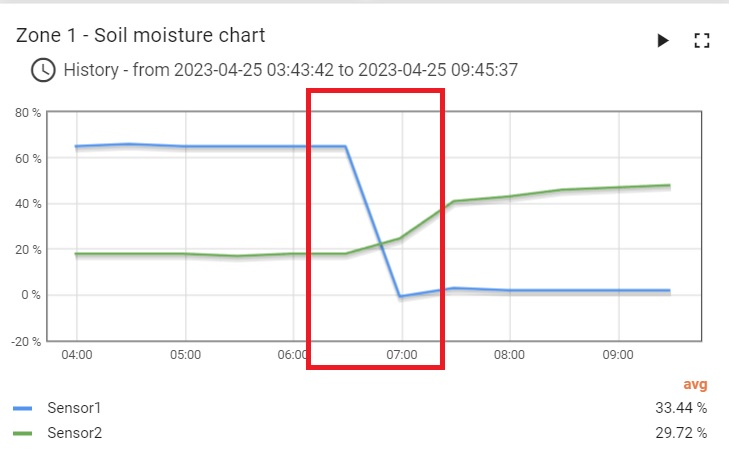
\includegraphics[width=0.9\textwidth]{./Figures/chapter4/soil_chart.jpg}
		\caption{Vista del historial de humedad del suelo.}
		\label{fig:temp_graph}
     \end{subfigure}
          \hfill
     \begin{subfigure}[b]{0.80\textwidth}
		\centering
		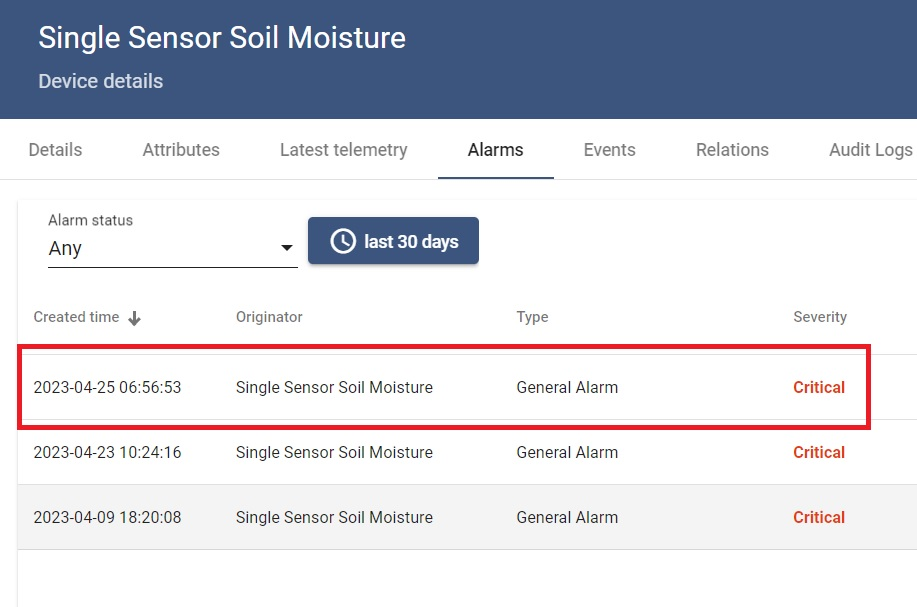
\includegraphics[width=0.80\textwidth]{./Figures/chapter4/soil_alarm.jpg}
		\caption{Alarmas generadas al superar los límites.}
		\label{fig:temp_alarm}
     \end{subfigure}
     \hfill
        \caption[Generación de alarmas por exceso de temperatura]{Generación de alarmas por exceso de temperatura.}
        \label{fig:tb_concurrencia}
\end{figure}


\section{Comparativa con el estado de arte}
\label{sec:Comparativa con el estado de arte}

